\numberwithin{figure}{section}

\chapter{Conception du systeme}

\section{Introduction}

Ce chapitre presente la conception du systeme FinderrLink. L'objectif est de donner une vision claire du fonctionnement general de la plateforme avant de passer a la realisation technique. Pour cela, trois diagrammes UML sont utilises : le diagramme de cas d'utilisation, le diagramme de classes et le diagramme de composants.

Le diagramme de cas d'utilisation permet de comprendre les interactions entre les acteurs et les principales fonctionnalites de la plateforme. Le diagramme de classes montre la structure interne du systeme a travers les entites principales et leurs relations. Enfin, le diagramme de composants presente l'organisation technique globale de l'application et les echanges entre ses differentes parties.

\section{Diagramme de cas d'utilisation}

Le diagramme de cas d'utilisation ci-dessous presente les principales actions possibles dans FinderrLink. Il permet de visualiser les roles des differents acteurs et les fonctionnalites accessibles selon chaque profil utilisateur.

\begin{figure}[H]
\centering
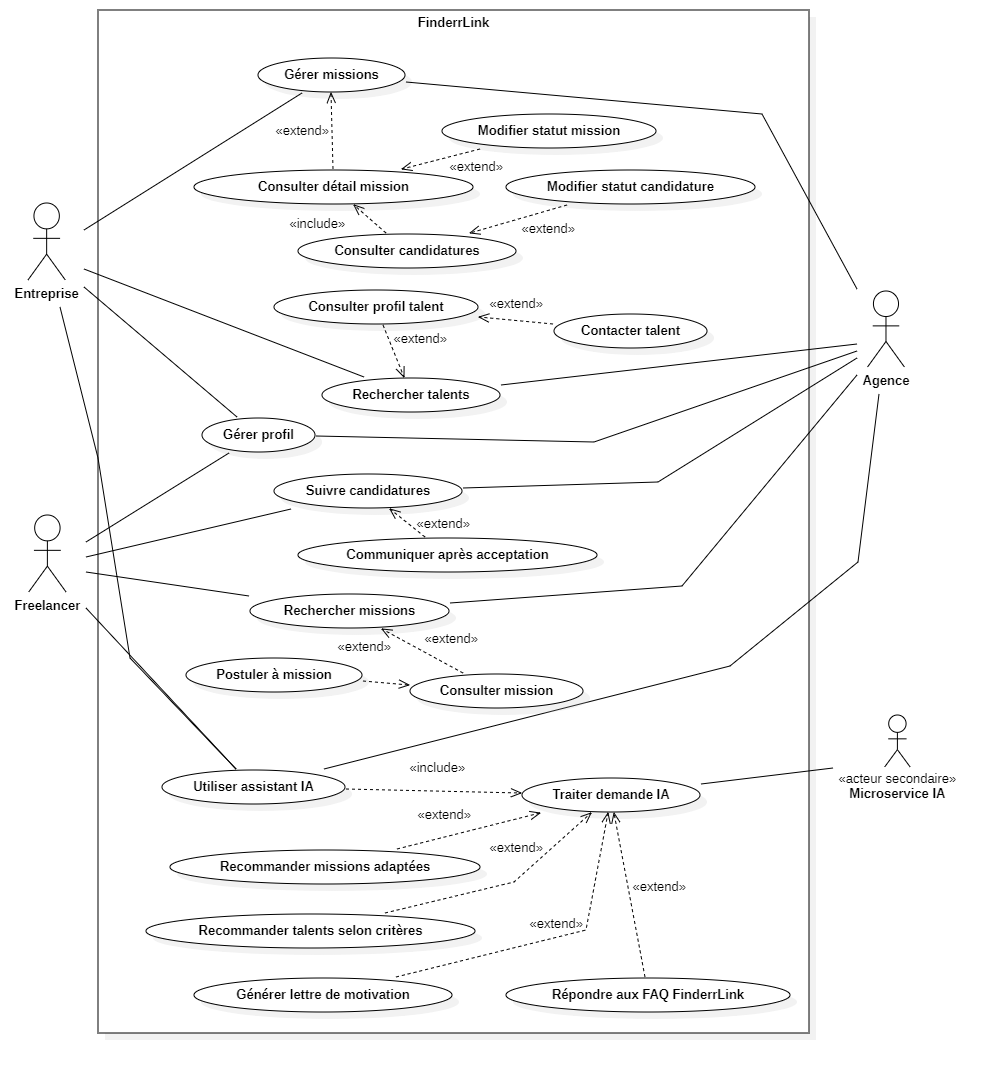
\includegraphics[width=0.95\textwidth]{./figures/UseCaseDiagram1.png}
\caption{Diagramme de cas d'utilisation - FinderrLink}
\label{fig:usecase_diagram_finderrlink}
\end{figure}

\subsection{Explication du diagramme de cas d'utilisation}

Le rectangle represente le systeme FinderrLink. Les acteurs places a l'exterieur du rectangle representent les utilisateurs ou services qui interagissent avec la plateforme. Les ovales representent les fonctionnalites principales.

Le freelance peut rechercher des missions, consulter une mission, postuler, suivre ses candidatures et communiquer apres acceptation. L'entreprise peut gerer ses missions, consulter les candidatures, modifier leur statut, rechercher des talents et contacter un talent. L'agence possede un role particulier, car elle peut publier des missions comme une entreprise et postuler a des missions comme un freelance.

Les relations \texttt{<<include>>} indiquent qu'une action contient obligatoirement une autre action. Les relations \texttt{<<extend>>} indiquent qu'une action peut completer une autre action selon le contexte. Par exemple, utiliser l'assistant IA inclut le traitement de la demande IA, tandis que recommander des missions adaptees ou generer une lettre de motivation sont des extensions possibles du traitement IA.

\section{Diagramme de classes UML}

Le diagramme de classes ci-dessous represente la structure principale de FinderrLink. Il montre les entites importantes du systeme, notamment les utilisateurs, les missions, les candidatures, les conversations, les notifications, les categories et la partie liee a l'assistant IA.

\begin{figure}[H]
\centering
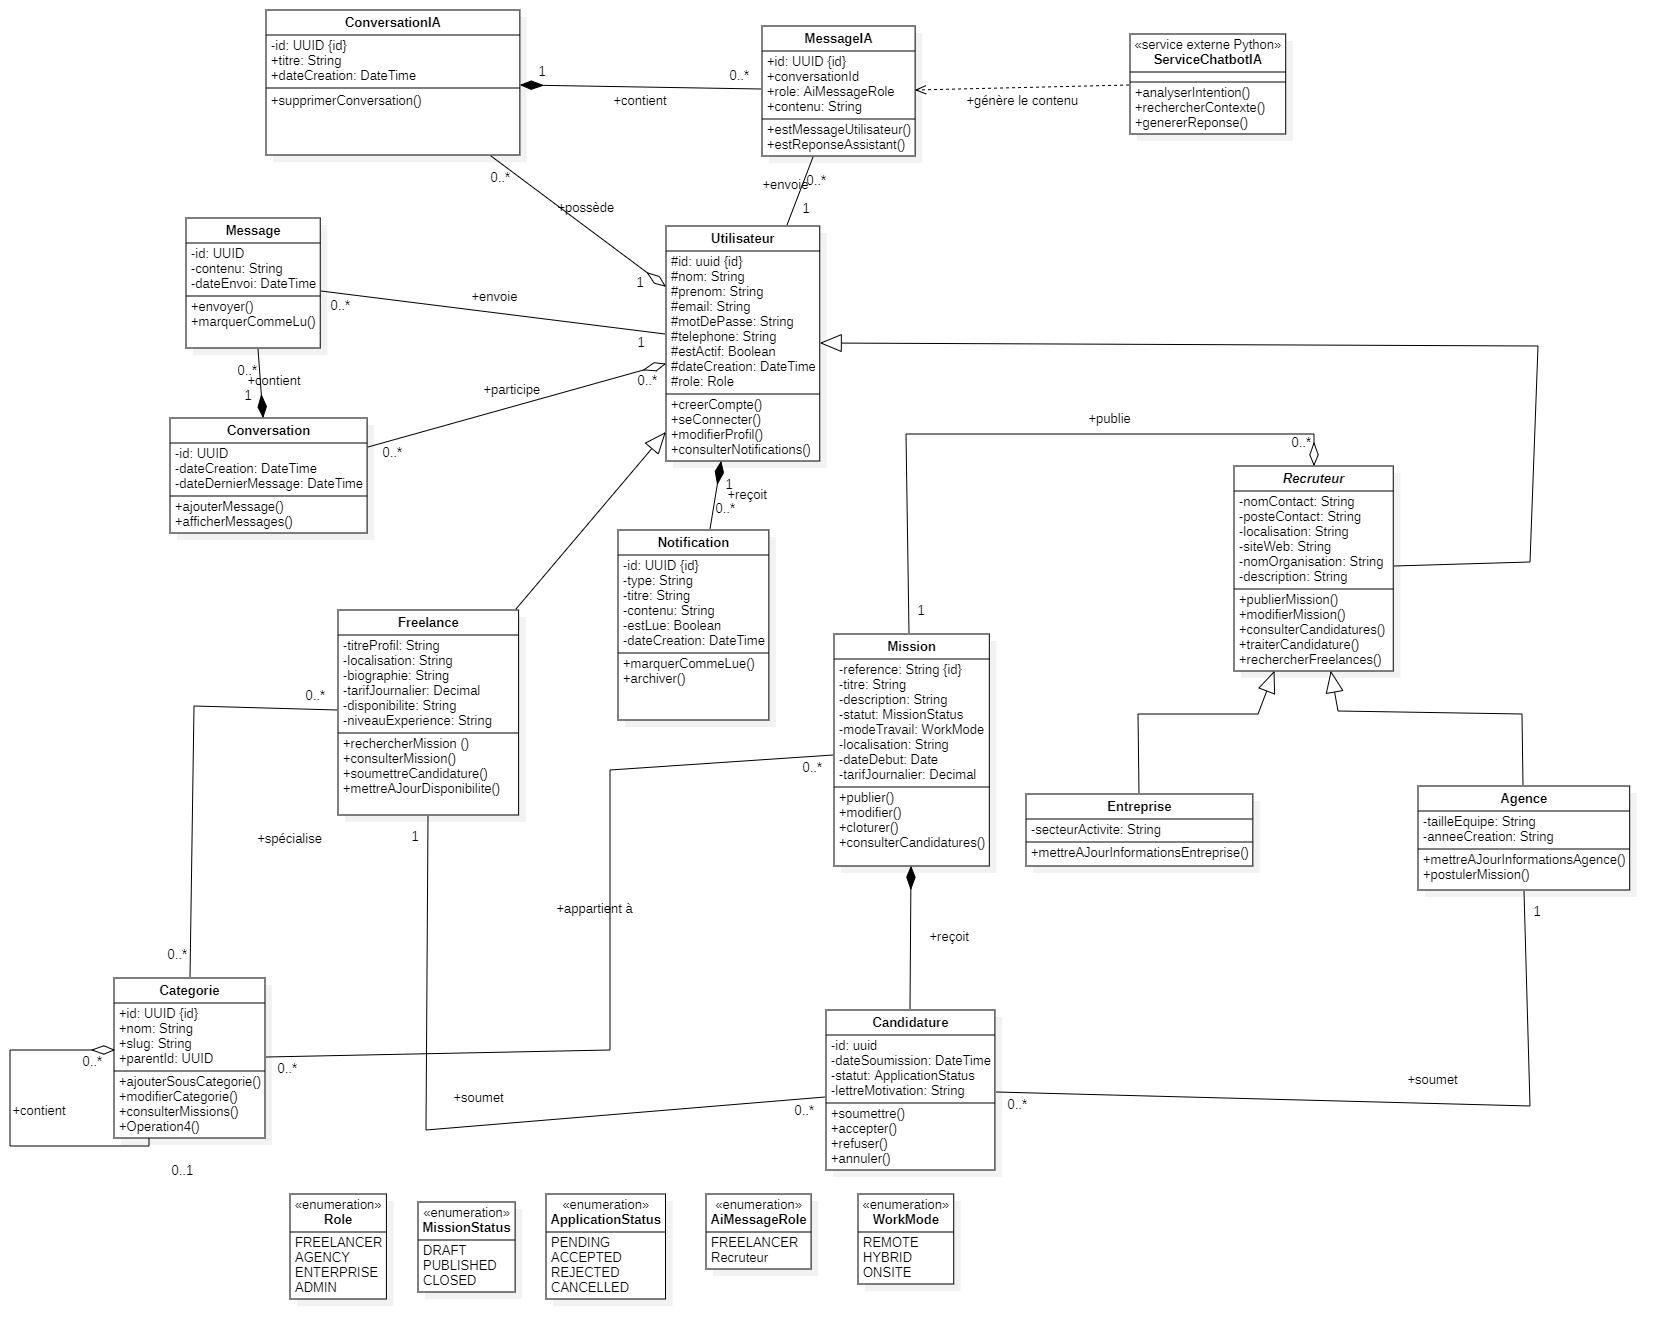
\includegraphics[width=1\textwidth]{./figures/ClassDiagram1.png}
\caption{Diagramme de classes UML - FinderrLink}
\label{fig:class_diagram_finderrlink}
\end{figure}

\subsection{Cle de lecture du diagramme de classes}

Une classe UML est representee par un rectangle divise en trois parties : le nom de la classe, les attributs et les methodes. Les attributs representent les donnees stockees, tandis que les methodes representent les actions possibles.

Le symbole \textbf{+} indique un element public. Le symbole \textbf{-} indique un element prive. Le symbole \textbf{\#} indique un element protege. Ces symboles permettent de preciser le niveau d'acces aux donnees et aux methodes.

L'heritage permet de representer une specialisation. Dans ce diagramme, les classes \textbf{Freelance}, \textbf{Recruteur}, \textbf{Entreprise} et \textbf{Agence} sont liees a la classe \textbf{Utilisateur}. Cela signifie que ces classes partagent des informations communes, comme le nom, l'email, le mot de passe, le telephone et le role.

L'agregation represente une relation souple entre deux classes. Les objets peuvent exister separement. La composition represente une relation plus forte, ou un element depend directement d'un autre. Par exemple, une conversation contient des messages, et une mission peut etre liee a plusieurs candidatures.

Les enumerations representent des listes de valeurs fixes. Elles permettent d'eviter les valeurs incoherentes. Par exemple, \textbf{Role} definit les types d'utilisateurs, \textbf{MissionStatus} definit l'etat d'une mission, \textbf{ApplicationStatus} definit le statut d'une candidature, et \textbf{WorkMode} definit le mode de travail.

\subsection{Explication simplifiee des classes principales}

La classe \textbf{Utilisateur} represente la base commune de tous les comptes. La classe \textbf{Freelance} represente un utilisateur qui cherche des missions et peut postuler. La classe \textbf{Recruteur} represente un utilisateur qui publie des missions et recherche des talents. Elle sert de base aux classes \textbf{Entreprise} et \textbf{Agence}.

L'entreprise publie des missions et consulte les profils freelances. L'agence possede un role hybride : elle peut publier des missions comme une entreprise, mais aussi postuler a des missions comme un freelance. Cette difference justifie la mise en place d'une gestion precise des roles et permissions.

La classe \textbf{Mission} represente une opportunite publiee sur la plateforme. La classe \textbf{Candidature} permet de suivre le lien entre un candidat et une mission. Les classes \textbf{Conversation} et \textbf{Message} representent la messagerie entre utilisateurs. Les classes \textbf{ConversationIA}, \textbf{MessageIA} et \textbf{ServiceChatBotIA} representent la partie assistant intelligent.

\section{Diagramme de composants}

Le diagramme de composants ci-dessous presente l'architecture technique globale de FinderrLink. Il montre les principaux blocs logiciels de la plateforme et la maniere dont ils communiquent entre eux.

\begin{figure}[H]
\centering
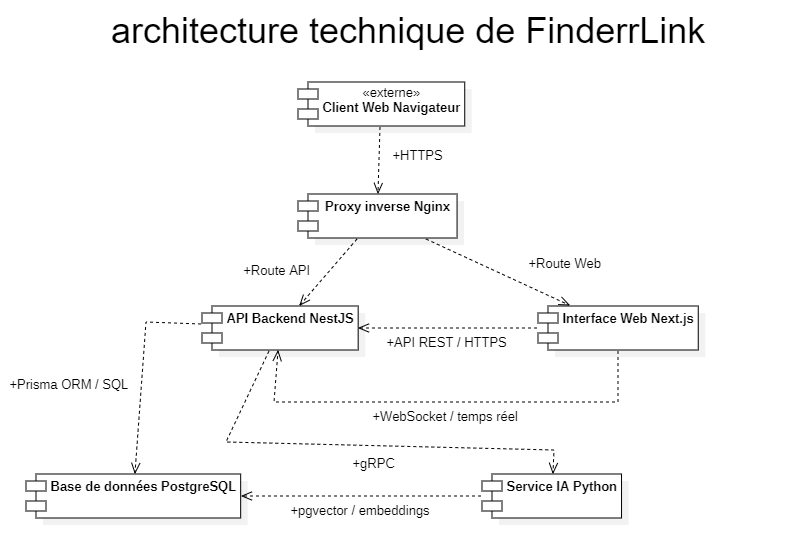
\includegraphics[width=0.95\textwidth]{./figures/ComponentDiagram1.png}
\caption{Diagramme de composants - FinderrLink}
\label{fig:component_diagram_finderrlink}
\end{figure}

\subsection{Explication du diagramme de composants}

Le client web navigateur represente l'utilisateur qui accede a la plateforme depuis un navigateur. Toutes les requetes passent d'abord par le proxy inverse Nginx, qui joue le role d'intermediaire entre l'utilisateur et les services internes.

L'interface web Next.js represente la partie frontend de l'application. Elle est responsable de l'affichage des pages, de l'experience utilisateur et de l'interaction avec les differents profils. L'API Backend NestJS represente la partie serveur. Elle contient la logique metier, la gestion des utilisateurs, des missions, des candidatures, des notifications et des communications avec les autres services.

La base de donnees PostgreSQL assure la persistance des donnees. Elle stocke les utilisateurs, les profils, les missions, les candidatures, les messages et les notifications. Le service IA Python represente le microservice intelligent utilise par FinderrLink pour traiter les demandes liees a l'assistant IA, comme la recherche de missions adaptees, la recommandation de talents ou la generation de reponses.

Ce diagramme montre que FinderrLink est organise selon une architecture separee en plusieurs composants. Cette separation facilite la maintenance, le deploiement, l'evolutivite et l'integration future de nouveaux services.
\section{Diagramme d'activite du service IA}

Le diagramme d'activite suivant presente le fonctionnement general du service d'intelligence artificielle integre dans FinderrLink. Ce diagramme permet de comprendre comment une demande utilisateur est analysee, filtree, traitee puis transformee en reponse avant d'etre retournee au backend de l'application.

\begin{landscape}
\begin{figure}[H]
\centering
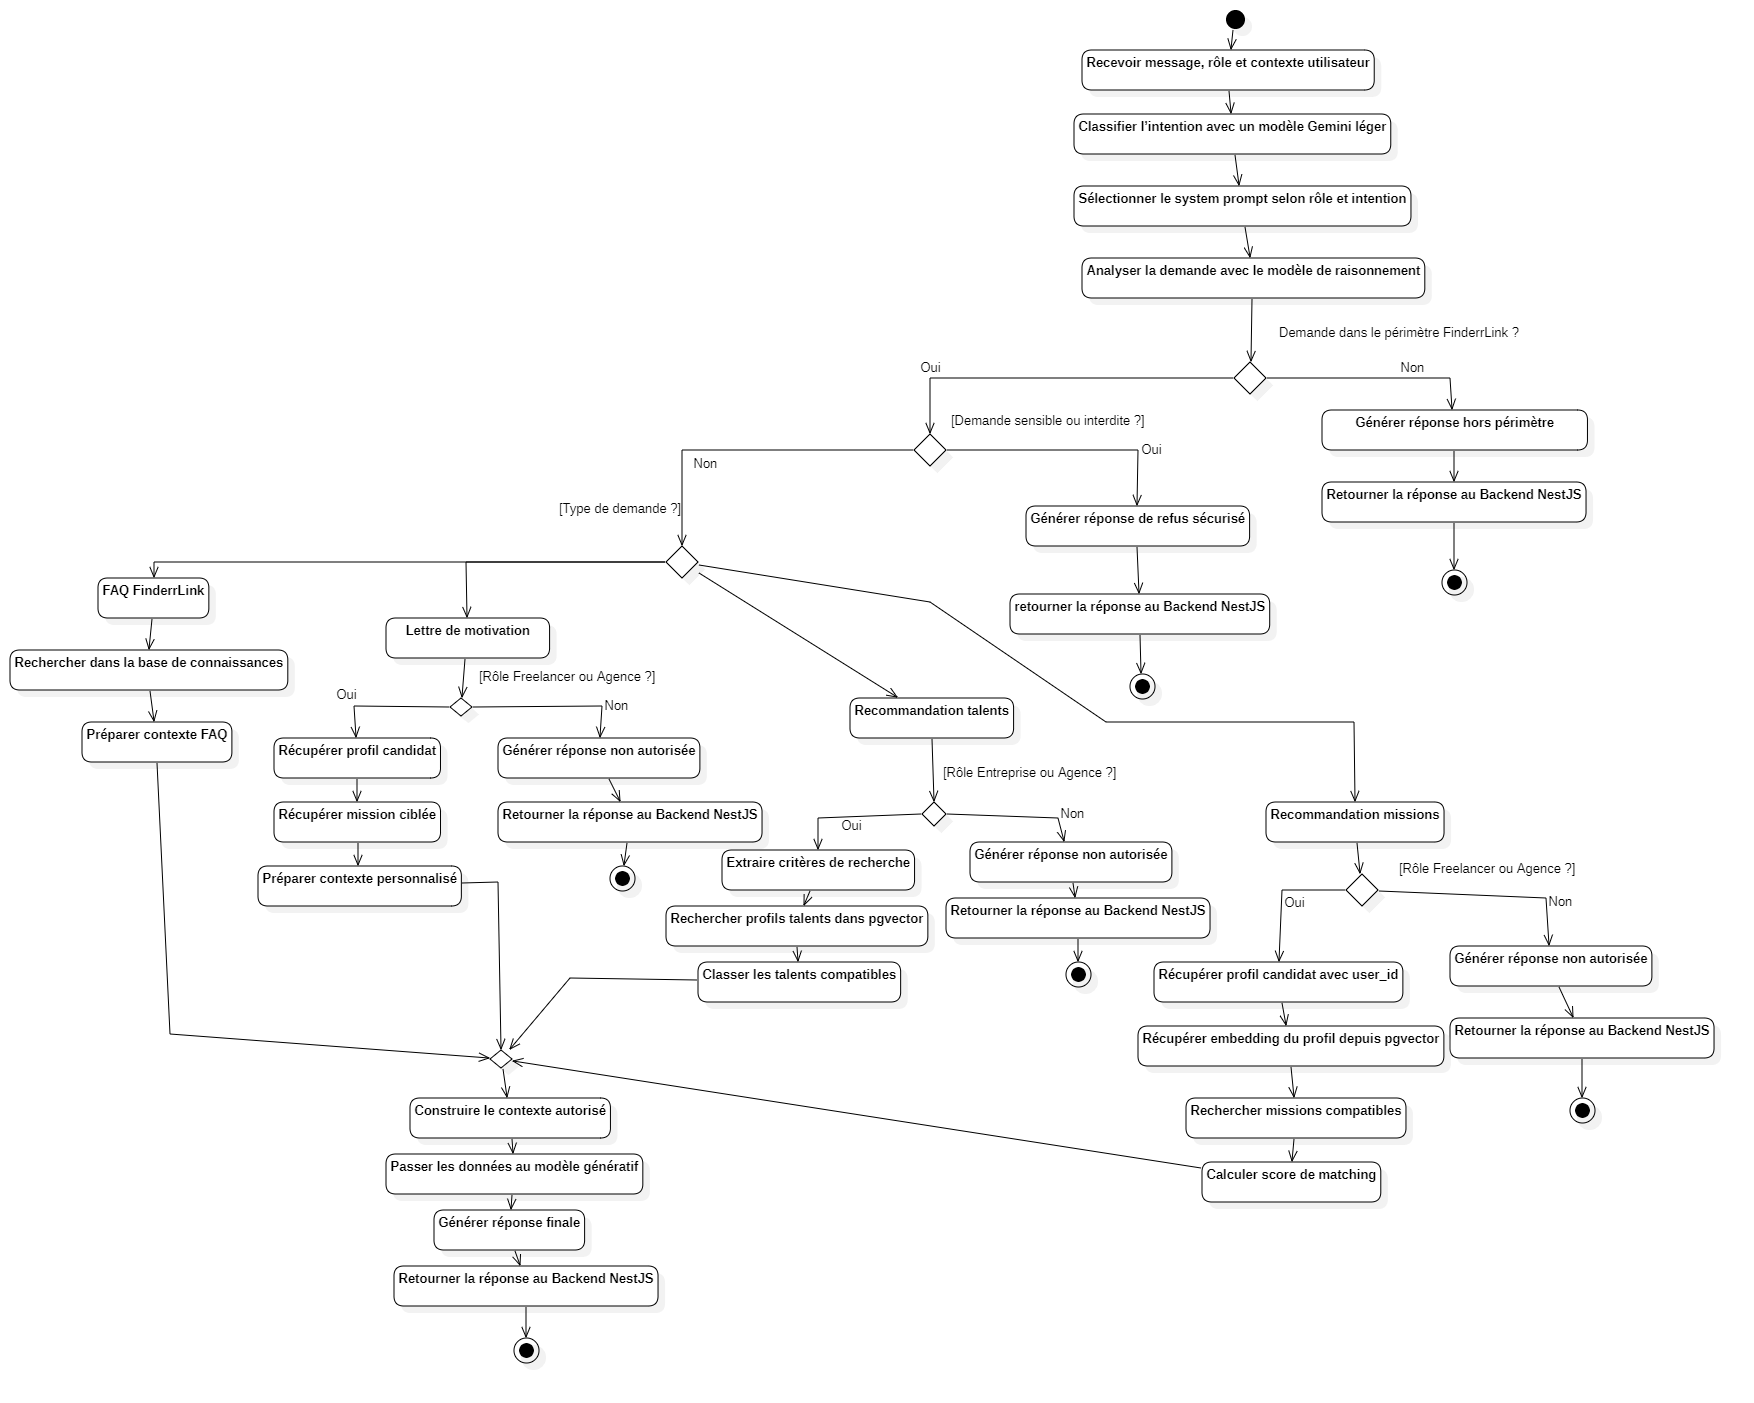
\includegraphics[width=0.95\linewidth]{./figures/ActivityDiagram1.png}
\caption{Diagramme d'activite du service IA - FinderrLink}
\label{fig:activity_diagram_ai_finderrlink}
\end{figure}
\end{landscape}

\subsection{Explication du diagramme d'activite IA}

Le processus commence par la reception du message de l'utilisateur avec son role et son contexte. Ces informations sont importantes, car les reponses de l'assistant doivent respecter les droits de chaque type d'utilisateur. Par exemple, un freelance ne doit pas acceder aux memes informations qu'une entreprise ou qu'une agence.

La premiere etape consiste a classifier l'intention de la demande a l'aide d'un modele Gemini leger. Cette classification permet d'identifier le type de besoin exprime par l'utilisateur, comme une recherche de missions, une recommandation de talents, une generation de lettre de motivation ou une question FAQ. Ensuite, le systeme selectionne le system prompt adapte au role et a l'intention afin d'encadrer correctement la reponse de l'assistant.

Apres cette premiere analyse, la demande est transmise a un modele de raisonnement plus avance. Ce modele verifie si la demande entre dans le perimetre de FinderrLink et si elle respecte les regles de securite. Si la demande est hors perimetre, le systeme genere une reponse adaptee sans acceder aux donnees internes. Si la demande est interdite ou non autorisee, une reponse de refus securisee est retournee.

Lorsque la demande est valide, le systeme suit un traitement specifique selon son type. Pour une recommandation de missions, le service recupere le profil du candidat, recherche les missions compatibles dans la base vectorielle et calcule un score de matching. Pour une recommandation de talents, il extrait les criteres de recherche, interroge les profils disponibles et classe les talents compatibles. Pour une lettre de motivation, il recupere le profil du candidat et la mission ciblee afin de construire un contexte personnalise. Pour une question FAQ, il recherche la reponse dans la base de connaissances de FinderrLink.

Enfin, les donnees autorisees sont transmises au modele generatif afin de produire une reponse finale claire et adaptee. Cette reponse est ensuite retournee au backend NestJS, qui se charge de l'envoyer a l'interface utilisateur. Ce fonctionnement montre que le service IA de FinderrLink ne se limite pas a generer du texte : il applique aussi une logique de classification, de controle d'acces, de recherche contextuelle et de generation securisee.

\section{Conclusion}

Cette conception permet de mieux comprendre l'organisation generale de FinderrLink. Le diagramme de cas d'utilisation montre les principales interactions entre les acteurs et la plateforme. Le diagramme de classes presente la structure interne du systeme. Le diagramme de composants montre l'architecture technique globale, composee du client web, du proxy Nginx, du frontend Next.js, du backend NestJS, de la base de donnees PostgreSQL et du service IA Python.
